\section{Data Profiling and Cleansing}
\subsection{Data Profiling}

The dataset has 7043 rows and 21 columns which include informations about :
\begin{longtable}{p{0.25\textwidth}p{0.65\textwidth}}
\caption{Description of each column.}
\label{tab:columndesc}
\endfirsthead
\hline
Column & Description\\ \hline
customerID & Represents Unique Id Number of each customer (do not give any useful informations) \\
gender & Represents the customer gender \\
SeniorCitizen & Whether the customer is a senior citizen or not (1, 0) \\
Partner & Categorical data, identifies whether the customer has a partner or not (Yes, No)\\
Dependents & Whether the customer has dependents or not (Yes, No) \\
tenure & Number of months the customer has stayed with the company\\
PhoneService & Whether the customer has a phone service or not (Yes, No)\\
MultipleLines & Whether the customer has multiple lines or not (Yes, No, No phone service)\\
InternetService & Customer’s internet service provider (DSL, Fiber optic, No)\\
OnlineSecurity & Whether the customer has online security or not (Yes, No, No internet service)\\
OnlineBackup & Whether the customer has online backup or not (Yes, No, No internet service)\\
DeviceProtection & Whether the customer has device protection or not (Yes, No, No internet service)\\
TechSupport & Whether the customer has tech support or not (Yes, No, No internet service)\\
StreamingTV & Whether the customer has streaming TV or not (Yes, No, No internet service)\\
 StreamingMovies & Whether the customer has streaming movies or not (Yes, No, No internet service)\\
 Contract & The contract term of the customer (Month-to-month, One year, Two year)\\
 PaperlessBilling & Whether the customer has paperless billing or not (Yes, No)\\
 PaymentMethod & The customer’s payment method (Electronic check, Mailed check, Bank transfer/automatic, Credit card/automatic)\\
 MonthlyCharges & The amount charged to the customer monthly\\
TotalCharges & The total amount charged to the customer\\
 Churn &Target variable, define whether the customer churns or not (Yes or No)\\ \hline
\end{longtable}
One can clearly see from Table \ref{tab:columndesc} that most columns (17) are categorical variables except customerID, tenure, MontlyCharges, and TotalCharges. The customerID variable is feature that represents unique Id number of each customer (in total has 7043 unique values) hence it won't give any useful informations and will be dropped from analysis  meanwhile tenure, MonthlyCharges and TotalCharges are considered as numerical variables.



\subsection{Data Cleansing}
It's important to eliminate all missing values and anomalies from the data before it will be analyzed further. In this telco customer dataset, TotalCharges is the only column where a few of missing values are detected.
\begin{figure}[tbph]
	\centering
	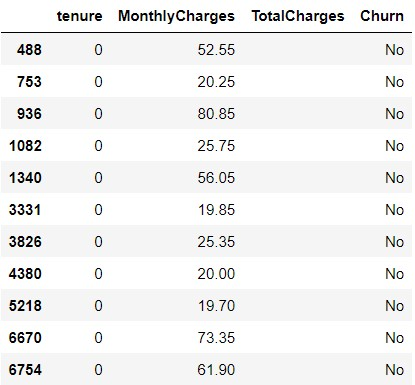
\includegraphics[width=0.6\linewidth]{figures/miss_values}
	\caption{All missing values detected in TotalCharges match 0 tenure period.}
	\label{fig:missvalues}
\end{figure}

There are in total 11 rows with missing value found in TotalCharges column and the reason behind these missing values is actually related to 0 tenure month (there are also 11 rows with 0 tenure). In addition, these rows with 0 period of tenure may emphasize the customer that has just signed up for the telecom service within the last month. Since they won't provide any useful information (the customers have just signed up) and the amount of rows are only 11, i.e 0.1\% of total rows, these rows will be eliminated and not included in the analysis.

Another thing one should be wary of before doing the analysis is the outlier.  An outlier is a value that deviates extremely from the rest observations within the sample data.  It may indicate bad and wrong observations or anomalies that need to be eliminated from the data. However, there are certain circumstances that outliers can reveal insights into special cases within the data that one may not otherwise notice. The best practice to detect the outlier is to use boxplot and it is shown in Figure \ref{fig:outlier1} that there is no outlier in the dataset.
\begin{figure}[tbph]
	\centering
	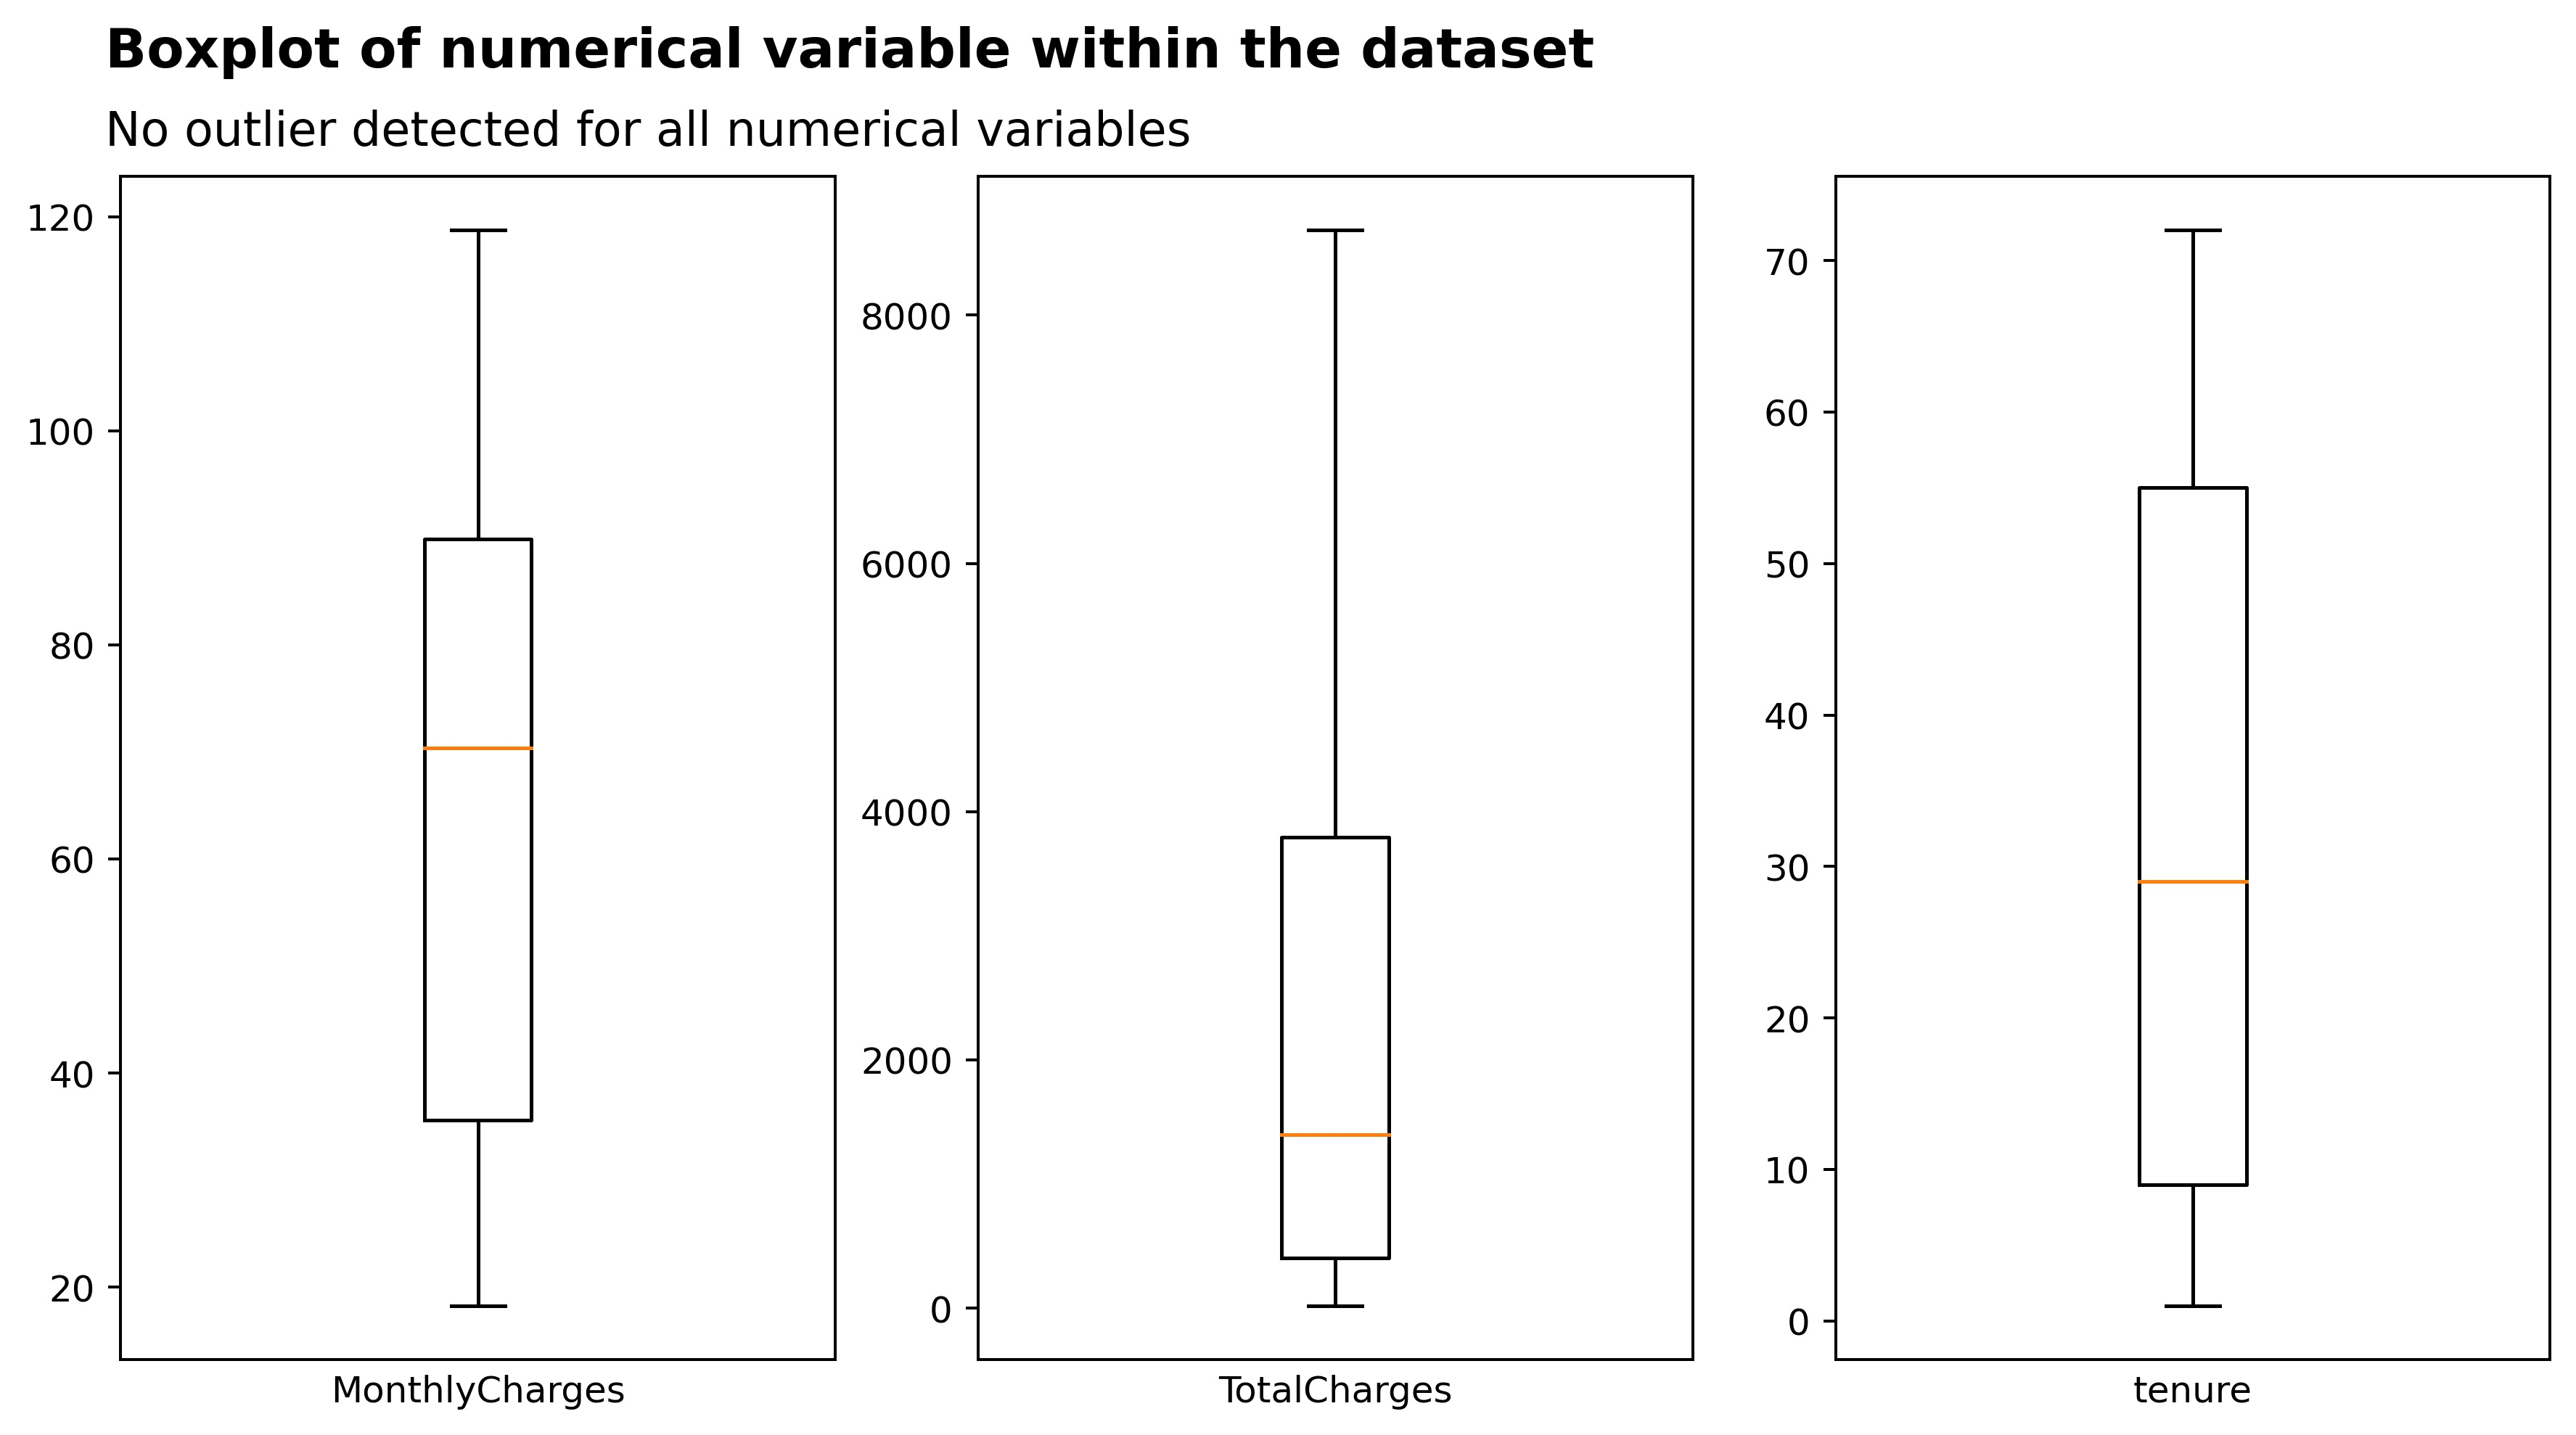
\includegraphics[width=1\linewidth]{figures/outlier1}
	\caption{No outlier found in the boxplots of MonthlyCharges, TotalCharges, and tenure.}
	\label{fig:outlier1}
\end{figure}

